% Mathe Formelsammlung für HM1 SoSe 2011
% 2 Seiten

% Dokumenteinstellungen
% ======================================================================	

% Dokumentklasse (Schriftgröße 6, DIN A4, Artikel)
\documentclass[6pt,a4paper]{scrartcl}

% Pakete laden
\usepackage[utf8]{inputenc}		% Zeichenkodierung: UTF-8 (für Umlautge)   
\usepackage[german]{babel}		% Deutsche Sprache
\usepackage{multicol}			% Spaltenpaket
\usepackage{amsmath}
\usepackage{amssymb}
\usepackage{esint}				% erweiterte Integralsymbole
\usepackage{multicol}			% ermöglicht Seitenspalten  
\usepackage{wasysym}			% Blitz
\usepackage{graphicx}
\usepackage{gensymb}
\usepackage{svg}

% Seitenlayout und Ränder:
\usepackage{geometry}
\geometry{a4paper, landscape, left=6mm,right=6mm, top=6mm, bottom=6mm} 
	
% Schriftart SANS für bessere Lesbarkeit bei kleiner Schrift
\renewcommand{\familydefault}{\sfdefault} 


% Custom Commands
\renewcommand{\thesubsection}{\arabic{subsection}}
\newcommand{\me}[1]{\ensuremath{\left\{#1\right\}}}
\newcommand{\dme}[2]{\ensuremath{\left\{#1\,\vert\,#2 \right\}}}
\newcommand{\abs}[1]{\ensuremath{\left\vert#1\right\vert}}
\newcommand{\un}[1]{\; \unit{#1} }
\newcommand{\unf}[2]{\;\left[ \unitfrac{#1}{#2} \right]}
\newcommand{\norm}[2][\relax]{\ifx#1\relax \ensuremath{\left\Vert#2\right\Vert}\else \ensuremath{\left\Vert#2\right\Vert_{#1}}\fi}
\newcommand{\enbrace}[1]{\ensuremath{\left(#1\right)}}
\newcommand{\nira}[1]{\ensuremath{\overset{n \rightarrow \infty}{\longrightarrow}}}
\newcommand{\os}[2]{\ensuremath{\overset{#1}{#2}}}
\makeatletter
\newcommand{\Ra}[0]{\ensuremath{\Rightarrow}}
\newcommand{\ra}[0]{\ensuremath{\rightarrow}}
\newcommand{\gk}[1]{\ensuremath{\left\lfloor#1\right\rfloor}}
\newcommand{\sprod}[2]{\ensuremath{%
  \setbox0=\hbox{\ensuremath{#2}}
  \dimen@\ht0
  \advance\dimen@ by \dp0
  \left\langle #1\rule[-\dp0]{0pt}{\dimen@},#2\right\rangle}}
% Für Mengen
\newcommand{\N}{\ensuremath{\mathbb N}}
\newcommand{\R}{\ensuremath{\mathbb R}}
\newcommand{\C}{\ensuremath{\mathbb C}}
\newcommand{\Q}{\ensuremath{\mathbb Q}}
\newcommand{\Z}{\ensuremath{\mathbb Z}}

% Dokumentbeginn
% ======================================================================
\begin{document}
%\subsection{}
% ----------------------------------------------------------------------

% Aufteilung in Spalten
\begin{multicols}{4}
      
\subsection{Allgemeines} % (fold)
\label{sub:allgemeines}

Dreiecksungleichung \qquad \qquad \qquad
\begin{math}\begin{array}{l}
	\abs{x + y} \le \abs{x} + \abs{y} \\
	\abs{\abs{x}- \abs{y}} \le \abs{x-y} 
\end{array}\end{math} \\
Cauchy-Schwarz-Ungleichung: \qquad
\begin{math}\begin{array}{l}
\left| \sprod{x}{y} \right| \le \| x\| \cdot \| y\|
\end{array}\end{math} \\
\\
Arithmetische Summenformel \qquad
\begin{math}\begin{array}{l}
	\sum\limits_{k = 1}^{n}k = \frac{n (n+1)}{2}
\end{array}\end{math}  \\
\\
Geometrische Summenformel \qquad 
\begin{math}\begin{array}{l}
	\sum\limits_{k = 0}^{n}q^k = \frac{1 - q^{n+1}}{1-q}
\end{array}\end{math}\\
\\                                   
Bernoulli-Ungleichung \qquad \qquad \quad
\begin{math}\begin{array}{l}
	(1+a)^n \ge 1 + na
\end{array}\end{math}\\   
\\
Binomialkoeffizient \qquad \qquad \qquad
\begin{math}\begin{array}{l}
	\binom{n}{k} = \frac{n!}{k!(n-k)!}  \\
	\binom{n}{0} = \binom{n}{n} = 1
\end{array}\end{math}\\ 
\\                   
Binomische Formel \qquad \qquad \qquad 
\begin{math}\begin{array}{l}
	(a+b)^n = \sum\limits_{k = 0}^{n} \binom{n}{k} a^{n-k} b^{k}
\end{array}\end{math}   \\ 
\\
Logarithmus \qquad \qquad \qquad \qquad \quad
\begin{math}\begin{array}{l}
	\ln{x^k}=k \cdot \ln{x}
\end{array}\end{math}   \\ 
Exponentialfunktion \qquad \qquad \qquad
\begin{math}\begin{array}{l}
	\exp(x) = \sum\limits_{n = 0}^\infty \frac{x^n}{n!}
\end{array}\end{math}   \\ 
\\
Wichtige Zahlen: $\sqrt{2} = 1,41421$\quad $e = 2,71828$ \quad $\pi =  3,14159$

\paragraph{Fakultäten} % (fold)
\label{par:fakultaeten}
$n! = 1 \cdot 2 \cdot 3 \cdot \ldots \cdot n$ \qquad  $0! = 1! = 1$ 
		

% paragraph fakultäten (end)
% subsubsection subsection_name (end)
% subsection allgemeines (end)


\subsection{Mengen}
% ----------------------------------------------------------------------

Eine Zusammenfassung wohlunterschiedener Elemente zu einer Menge\\
explizite Angabe: $A=\{1;2;3\}$\\
Angabe durch Eigenschaft: $A=\lbrace n \in \N \vert 0<n<4 \rbrace$\\
\subsubsection{Für alle Mengen A,B,C gilt:}
\begin{enumerate}\itemsep-1pt
\item $\emptyset \subseteq B $
\item $A \setminus (B \cup C) = (A \setminus B) \cap (A \setminus C)$
\item $(A \cap B) \cap C = A \cap (B \cap C)$\\
	$(A \cup B) \cup C = A \cup (B \cup C)$
\item $A \cap (B \cup C) = (A \cap B) \cup (A \cap C) \\
	A \cup (B \cap C) = (A \cup B) \cap (A \cup C)$
\end{enumerate}

\subsubsection{Offenheit}
Offen: \begin{enumerate}\itemsep-1pt
\item $\forall x \in X ~ \exists \delta > 0 : B_\delta(x)<X$
\item $\exists x \in \delta (\R^n\setminus X)$ mit $x \in (\R^n\setminus X)$
\end{enumerate}
Geschlossen: $\exists x \in \delta (\R^n\setminus X)$ mit $x \notin (\R^n\setminus X)$ \\
$\emptyset$ : beides \\

\subsubsection{Rationale Zahlen}
$\mathbb Q=\{\frac{p}{q}\ \vert\ p\in\mathbb Z; q\in\N\}$\\
\\
Jede rationale Zahl $\frac m n \in \mathbb Q$ hat ein Dezimaldarstellung.\\
$0,25\overline{54} =: a \rightarrow 10000a - 100a = 2554 -25 \Rightarrow a(9900) = 2529 \qquad \Rightarrow a = \frac{2529}{9900} = \frac{281}{1100}$

\subsection{Vollständige Induktion}
Behauptung: $f(n)=g(n)$ für $n_0 \le n \in \N$\\ 
IA: $n=n_0$: \quad Zeige $f(n_0)=g(n_0)=$wahr.\\
IV: Behauptung gilt für ein beliebiges $n\in\N$ \quad (Sei $f(n)=$wahr)\\
IS: $n \rightarrow n+1$: \quad Zeige $f(n+1)=\underset{=wahr}{f(n)}  \dotsc=g(n+1)$

\subsection{Komplexe Zahlen}
% ----------------------------------------------------------------------
Eine komplexe Zahl $z=a+b\mathbf{i},\ z\in \mathbb C a,b \in \R$ besteht aus einem Realteil $\Re(z)=a$ und einem Imaginärteil $\Im(z)=b$, wobei $\mathbf{i}=\sqrt{-1}$ die immaginären Einheit ist.
Es gilt: \quad $i^2 = -1$ \quad $i^4 = 1$ \\
\subsubsection{Kartesische Koordinaten}
Rechenregeln:\\
$z_1+z_2=(a_1+a_2)+(b_1+b_2)\mathbf{i}$\\
$z_1\cdot z_2=(a_1\cdot a_2-b_1\cdot b_2)+(a_1\cdot b_2+a_2\cdot b_1)\mathbf{i}$\\
\\
Konjugiertes Element von $z=a+b\mathbf{i}$:\\
$\overline{z}=a-b\mathbf{i}$\qquad \qquad \qquad \qquad \qquad \qquad \qquad \qquad $e^{\overline{ix}} = e^{-ix}$  \\
$z\overline{z}=|z|^2=a^2+b^2$\\
\\
Inverses Element:\\
$z^{-1}=\frac{\overline z}{\overline z z}=\frac{\overline z}{a^2+b^2}=\frac{a}{a^2+b^2} - \frac{b}{a^2+b^2}\mathbf{i}$ \\
\\
neutrales Element, zum Gleichungen lösen u.ä.: \\ 
$\frac{\overline{z}}{\overline{z}}=1$ \\
Bsp.: $z=\frac{x}{a+b i}=\frac{x}{a+bi}\cdot\frac{a-bi}{a-bi}=\frac{x\cdot(a-bi)}{a^2+b^2}$

\subsubsection{Polarkoordinaten}
$z=a+b\mathbf{i}\ne0$\ in Polarkoordinaten:\\
$z=r (\cos(\varphi)+\mathbf{i}\sin(\varphi))=r\cdot e^{\varphi \mathbf{i}}$\\
$r=|z|=\sqrt{a^2+b^2}\quad\varphi=\arg(z)=\begin{cases}+\arccos \left( \frac{a}{r}\right),  & b\ge0   \\  -\arccos \left( \frac{a}{r}\right), & b<0\end{cases}$ \\
Exponentialfunktion: $r\cdot e^{\varphi \mathbf{i}}=r (\cos(\varphi)+\mathbf{i}\sin(\varphi))$\\

\begin{description}\itemsep0pt
\item[Multiplikation:] $z_1\cdot z_2=r_1 * r_2 ( \cos ( \varphi_1 + \varphi_2) + \mathbf{i} \sin (\varphi_1 + \varphi_2))$
\item[Division:] $\frac{z_1}{z_2}=\frac{r_1}{r_2} ( \cos ( \varphi_1 - \varphi_2) + \mathbf{i} \sin (\varphi_1 - \varphi_2))$
\item[n-te Potenz:] $z^n=r^n\cdot e^{n\varphi \mathbf{i}}= r^n (\cos (n \varphi) + \mathbf{i} \sin (n \varphi))$
\item[n-te Wurzel:] $\sqrt[n]{z}= z_k = \sqrt[n]{r} \left(\cos \left(\frac{\varphi + 2k\pi}{n}\right) + \mathbf{i} \sin \left(\frac{\varphi + 2k\pi}{n}\right)\right) \\ k =0,1, \ldots, n-1$
\item[Logarithmus:] $\ln(z)=\ln(r) + \mathbf{i}(\varphi + 2k\pi)$ \quad (Nicht eindeutig!)
\end{description}
Anmerkung: Addition in kartesische Koordinaten umrechnen(leichter)!

\subsection{Funktionen}
Eine Funktion $f$ ist eine Abbildung, die jedem Element $x$ einer Definitionsmenge $D$ genau ein Element $y$ einer Wertemenge $W$ zuordnet.\\
$f:D\mapsto W,\ x \mapsto f(x):=y$\\
\\
\textbf{Injektiv}: $f(x_1)=f(x_2) \Rightarrow x_1=x_2$\\
\textbf{Surjektiv}: $\forall y\in W \exists x\in D:f(x)=y$\\ \quad (Alle Werte aus $W$ werden angenommen.)\\
\textbf{Bijektiv}: $f$ ist injektiv und surjektiv $\Rightarrow$ $f$ umkehrbar.

\subsubsection{Symmetrie einer Funktion $f$}
\textbf{Achsensymmetrie}(gerade Funktion): $f(x)=f(-x)$\\
\textbf{Punktsymmetrie}(ungerade Funktion): $f(x)=-f(-x)$\\
\\
Regeln für gerade Funktion $g$ und ungerade Funktion $u$:\\
$g_1 \pm g_2 = g_3$ \qquad $u_1 \pm u_2 = u_3$\\
$g_1 \cdot g_2=g_3$ \qquad $u_1 \cdot u_2 = g_3$ \qquad $u_1 \cdot g_1=u_3$ \\
Ist $f: \R \mapsto \R$ gerade und diffbar so ist $f'$ ungerade (nach Kettenregel). Selbes gilt umgekehrt für ungerade Funktionen.

\subsubsection{Konvex und konkav}
$f: C\mapsto\R$ für alle $x,y \in C \wedge t \in [0,1]$\\
Konvex: $f(tx+(1-t)y)\leq tf(x)+(1-t)f(y)$ \\
Konkav: $f(tx+(1-t)y)\geq tf(x)+(1-t)f(y)$ \\
streng/strikt für $x \neq y$ \\
Lineare Funktionen: beides, aber nicht strikt \\
falls Funktion 2 mal stetig diff'bar: \\
konvex: $f''(x)\geq 0 \forall x \in (a,b)$ \\
konkav: $f''(x)\leq 0 ~\forall x \in (a,b)$

\subsubsection{Extrema, Monotonie und Krümmung von $f$}
$f'(x_0)\overset{!}{=}0 \quad \begin{cases}f''(x_0)<0 \ \rightarrow \ \text{Maximum (lokal)} \\ f''(x_0)>0 \ \rightarrow \ \text{Minimum (lokal)}\end{cases} $\\
$f'(x) \underset{(>)}{^{\ge}} / \underset{(<)}{^{\le}} 0 \ \rightarrow$ \ $f$ (streng) Monoton steigend/fallend. $x\in[a,b]$\\
$f''(x) \underset{(>)}{^{\ge}} / \underset{(<)}{^{\le}} 0 \ \rightarrow$ \ $f$ (strikt) konvex/konkav. $x\in[a,b]$\\

\subsubsection{Asymptoten von $f$}
Horizontal: $c=\lim\limits_{x\ra \pm \infty} f(x)$\\
Vertikal: $\exists \text{ Nullstelle } a \text{ des Nenners }: \lim\limits_{x \rightarrow a^{\pm}} f(x) = \pm \infty$\\
Polynomasymptote $P(x)$: $f(x):=\frac{A(x)}{Q(x)}=P(x)+ \underset{\ra 0}{\frac{B(x)}{Q(x)}}$


\subsubsection{Wichtige Sätze für \underline{stetige} Fkt. $f: [a,b] \mapsto \R, f \mapsto f(x)$ }
\textbf{Zwischenwertsatz:} $\forall y \in [f(a),f(b)]\ \exists x\in [a,b]:f(x)=y$\\
\textbf{Mittelwertsatz:} Falls $f$ diffbar, dann $\exists \xi:f'(\xi)=\frac{f(b)-f(a)}{b-a}$\\
\textbf{Satz von Rolle:} Falls $f(a)=f(b)$, dann $\exists x_0: f' (x_0) = 0$\\
\textbf{Regel von L'Hospital}: (Falls $\exists$ ein Grenzwert) \\ $\lim\limits_{x \rightarrow a} \frac{f(x)}{g(x)} \rightarrow \left[ \frac{0}{0} \right] / \left[ \frac{\infty}{\infty} \right] = \lim\limits_{x \rightarrow a} \frac{f'(x)}{g'(x)}$

% ----------------------------------------------------------------------
\subsubsection{Polynome $P(x)\in\R[x]_n$}
$P(x)=\sum\limits_{i=0}^n a_ix^i=a_n x^n+a_{n-1} x^{n-1}+\dotsc+a_1x+a_0$ \\
Lösungen für $ax^2+bx+c=0$ \\
\begin{tabular}{l|l}
Mitternachtsformel:  &  Satz von Vieta:\\
$x_{1/2}=\frac{-b\pm\sqrt{b^2-4ac}}{2a}$  \quad & \quad   $x_1 + x_2 = - \frac{b}{a} \qquad x_1 x_2 = \frac{c}{a}$
\end{tabular}

\subsubsection{Trigonometrische Funktionen}
$f(t)=A\cdot \cos(\omega t + \varphi_0)=A\cdot \sin(\omega t + \frac{\pi}{2}+ \varphi_0)$
\begin{eqnarray*}
	\sin (-x) = -\sin (x)  \quad & \quad \cos (-x) = \cos (x) \\
	\sin^2 x + \cos^2 x = 1  \quad & \quad \tan x = \frac{\sin x}{\cos x}
\end{eqnarray*}
$e^{ix}=\cos(x)+i\sin(x)\\
e^{-ix}=\sin(x)-i\cos(x)$

\paragraph{Additionstheoreme} % (fold)
\label{par:additionstheoreme}
 \begin{eqnarray*}
    \sin \enbrace{x \pm y} = \sin x \cos y \pm \cos x \sin y \\
 	\cos \enbrace{x \pm y} = \cos x \cos y \mp \sin x \sin y \\
	\cos \enbrace{x - \frac{\pi}{2}} = \sin x \qquad \quad \sin \enbrace{x + \frac{\pi}{2}} = \cos x \\
	\sin 2x = 2 \sin x \cos x        \\
	\cos 2x = \cos^2 x - \sin^2 x = 2\cos^2 x - 1\\
	\tan(x\pm y)=\frac{\sin(x\pm y)}{\cos(x\pm y)}
 \end{eqnarray*}
% paragraph additionstheoreme (end)

$\begin{array}{c|c|c|c|c|c|c|c|c}
x & 0 & \frac{\pi}{6} & \frac{\pi}{4} & \frac{\pi}{3} & \frac{\pi}{2} & \pi & \frac{3}{2}\pi & 2 \pi \\ \hline
\sin & 0 & \frac{1}{2} & \frac{1}{\sqrt{2}} & \frac{\sqrt 3}{2} & 1 & 0 & -1 & 0 \\
\cos & 1 & \frac{\sqrt 3}{2} & \frac{1}{\sqrt 2} & \frac{1}{2} & 0 & -1 & 0 & 1 \\     
\tan & 0 & \frac{\sqrt{3}}{3}&	1				 &	\sqrt{3} & \lightning & 0 & \lightning & 0\\
\end{array}$

\subsubsection{Umkehrfunktion}
x(t): nach t auflösen\\

\subsection{Folgen}
% ----------------------------------------------------------------------
Eine Folge ist eine Abbildung $a: \N_0 \mapsto \R,\ n \rightarrow a(n) =: a_n$\\
explizite Folge: $(a_n)$ mit $a_n=a(n)$\\ rekursive Folge: $(a_n)$ mit $a_0=f_0,\  a_{n+1}=a(a_n)$\\

\subsubsection{Monotonie}
Im Wesentlichen gibt es 3 Methoden zum Nachweis der Monotonie:
\begin{enumerate}\itemsep0pt
\item $a_{n+1} - a_n \gtrless (=) 0$
\item $\frac{a_n}{a_{n+1}} \gtrless (=) 1$ \qquad $\lor$ \qquad $\frac{a_{n+1}}{a_n} \lessgtr (=) 1$
\item Vollständige Induktion
\end{enumerate}

\subsubsection{Konvergenz}
$(a_n)$ ist \emph{Konvergent} mit \emph{Grenzwert} $a$, falls: $\forall \epsilon > 0\, \exists N  \in \N_0:  \abs{a_n -a} < \epsilon  \forall n \ge N$\\
Eine Folge konvergiert gegen eine Zahl $a$:\ $(a_n) \overset{n \rightarrow \infty}{\longrightarrow} a$\\
\paragraph{Es gilt:}
\begin{itemize}\itemsep0pt
\item Der Grenzwert a einer Folge $(a_n)$ ist eindeutig.
\item Ist $(a_n)$ Konvergent, so ist $(a_n)$ beschränkt
\item Ist $(a_n)$ unbeschränkt, so ist $(a_n)$ divergent.
\item \emph{Das Monotoniekriterium}: Ist $(a_n)$ beschränkt und monoton, so konvergiert $(a_n)$
\item \emph{Das Cauchy-Kriterium:} Eine Folge $(a_n)$ konvergiert gerade dann, wenn: \\ $\forall \epsilon >0 \, \exists \,  N \in \N_0: \abs{a_n - n_m} < \epsilon \, \forall n, m \ge N$
\end{itemize}
Regeln für konvergente Folgen $(a_n) \overset{n \rightarrow \infty}{\longrightarrow} a$ und $(b_n) \overset{n \rightarrow \infty}{\longrightarrow} b$:\\
$\begin{array}{lll}
(a_n+b_n) \overset{n \rightarrow \infty}{\longrightarrow} a+b & (a_n b_n) \overset{n \rightarrow \infty}{\longrightarrow} ab & (\frac{a_n}{b_n}) \overset{n \rightarrow \infty}{\longrightarrow} \frac{a}{b}\\
(\lambda a_n) \overset{n \rightarrow \infty}{\longrightarrow} \lambda a & (\sqrt{a_n}) \overset{n \rightarrow \infty}{\longrightarrow} \sqrt{a} & (|a_n|) \overset{n \rightarrow \infty}{\longrightarrow} |a|
\end{array}$

\subsubsection{Wichtige Regeln}
$a_n=q^n \quad \overset{n \rightarrow \infty}{\longrightarrow} \quad \begin{cases} 0 & |q|<1 \\ 1 & q=1 \\ \pm \infty & q < -1  \\  + \infty & q > 1\end{cases}$ \\
$a_n=\frac{1}{n^k}\rightarrow 0$ \qquad $\forall k \ge 1$\\ 
$a_n=\left(1+\frac{c}{n}\right)^n \rightarrow e^c$ \qquad \qquad \qquad $2^n \ge n^2$ \quad $\forall n\ge 4$





\subsection{Reihen}
% ----------------------------------------------------------------------
Harmonische Reihe:
\begin{itemize}\itemsep-2pt
\item $\sum\limits_{n=1}^\infty \frac{1}{n} = \infty$ 
\item allgemein: $\sum\limits_{n=1}^\infty \frac{-1^{n+1}}{n} = \ln 2$
\item alternierend: $\sum\limits_{n=1}^\infty \frac{1}{n^\alpha}$ \\
konvergiert für $\alpha > 1$ \quad divergiert für $\alpha \leq 1$
\end{itemize}
Geometrische Reihe: $\sum\limits_{n=0}^{\infty}q^n = \frac{1}{1-q} \quad|q|<1$ \\
\textbf{n = 0}, notfalls Index verschieben

\subsubsection{Konvergenzkriterien}
$\sum\limits^{\infty}_{n = 0} a_n$ divergiert, falls $a_n \not \rightarrow 0$ oder\\
Minorante:$\exists \sum\limits^{\infty}_{n = 0} b_n (div) \quad \land \quad a_n \ge b_n \ \forall n\ge n_0$\\[0.6em] 
Leibniz: $\sum\limits^{\infty}_{n = 0}(-1)^n a_n$ konvergiert falls $a_n$ monoton fallende Nullfolge\\
oder Majorante: $\exists \sum\limits^{\infty}_{n = 0} b_n = b \quad \land \quad a_n \le b_n \ \forall n\ge n_0$\\
\\
Absolute Konvergenz ($\sum\limits^\infty_{n=0} |a_n|=a$ konvergiert), falls:\\
Majorante: $\exists \sum\limits^{\infty}_{n = 0} b_n = b \quad \land \quad |a_n| \le b_n \quad \forall n\ge n_0$\\
Quotienten und Wurzelkriterium:
\begin{eqnarray*}
	\rho := \lim_{n \rightarrow \infty} \abs{\frac{a_{n+1}}{a_n}} \qquad \lor \qquad \rho := \lim_{n \rightarrow \infty} \sqrt[n]{\abs{a_n}}\\
	\text{Falls} 
	\begin{cases}
		\rho < 1 \Ra  ~\sum\limits^\infty_{n=0} a_n \text{ konvergiert absolut} \\
		\rho > 1 \Ra  ~\sum\limits^\infty_{n=0} a_n \text{ divergiert} \\
		\rho = 1 \Ra ~ \sum\limits^\infty_{n=0} a_n \text{ keine Aussage möglich}
	\end{cases}
\end{eqnarray*}
\\


\subsection{Potenzreihen} % (fold)
% ----------------------------------------------------------------------
\begin{equation*}
f(x)=\sum_{n=0}^\infty a_n \cdot (x-a)^n = \sum_{n=0}^\infty a_n q^n
\end{equation*}
Konvergenz:\\
$\abs{\frac{a_{n+1} (x-a)^{n+1}}{a_n (x-a)^n}} = \abs{\frac{a_{n+1}}{a_n}}\abs{x-a} \overset{n \rightarrow \infty}{\rightarrow} q \cdot \abs{x -a}$\\
Falls $\begin{cases}  \abs z = \abs{x-a} < \frac{1}{q} & \text{ konvergiert absolut}\\
	\abs z = \abs{x-a} > \frac{1}{q} & \text{ divergiert} \\
	\abs z = \abs{x-a} = \frac{1}{q}  & \text{ keine Aussage möglich (Wert auf Radius)}
	\end{cases}$\\
Konvergenzradius: $R=\frac{1}{q}$\\
$R = \lim\limits_{n \rightarrow \infty} \abs{\frac{a_n}{a_{n+1}}}=\frac{1}{\lim\limits_{n\rightarrow \infty}\sqrt[n]{\abs{a_n}}}$ \\
Mittelpunkt s: $q$ nach x auflösen \\
Intervall: $I=(s-R, s+R)$ 

\label{sub:potenzreihen}
 \begin{eqnarray*}
 	e^z = \sum_{n = 0}^{\infty} \frac{z^n}{n!}\\
	\sin (z) = \sum_{n = 0}^{\infty} (-1)^n \frac{z^{2n +1}}{(2n +1)!} = \frac{e^{iz} - e^{-iz}}{2i} \\
	\cos (z) = \sum_{n = 0}^{\infty} (-1)^n \frac{z^{2n}}{(2n)!} = \frac{e^{iz} + e^{-iz}}{2}\\
 \end{eqnarray*}

$\limsup=\max(\lim)$ \\
z.B. bei $a_n=(2+(-1)^n)^n \\
\Rrightarrow$ Fallunterscheidung (gerade/ungerade) + R=$\frac{1}{\limsup(\sqrt[n]{|a_n|})}$
% subsection potenzreihen (end)


\subsection{Ableitung und Integral}
$f$ diffbar, falls $f$ stetig und $\underset{h\rightarrow 0}{\lim}\frac{f(x_0+h)-f(x_0)}{h}=f'(x)$ exist. \\
Ableitung nur auf offenen Intervall.
\subsubsection{Ableitungsregeln:}
Linearität: $(\lambda f + \mu g)' (x) = \lambda f'(x) + \mu g'(x)$ \quad $\forall \lambda, \mu \in \R$ \\
Produktregel: $(f \cdot g)'(x) = f'(x) g(x) + f(x) g'(x)$\\
Quotientenregel$\enbrace{\frac{\text{NAZ}-\text{ZAN}}{\text{N}^2}}$: $\enbrace{\frac{f}{g}}' (x) = \frac{g(x)f'(x) -f(x) g'(x)}{g(x)^2}$\\
Kettenregel: $\left( f(g(x)) \right)' = f'(g(x)) g'(x)$\\
Potenzreihe: $f: (\underbrace{-R+a, a+R}_{\subseteq D}) \mapsto \R, f(x) = \sum\limits_{n=0}^{\infty} a_n (x -a)^n$ \quad $\Rightarrow$ \quad $f'(x) = \sum\limits_{n=0}^{\infty} n a_{n} (x-a)^{n-1}$\\
\textbf{Tangentengleichung:} $y=f(x_0)+f'(x_0)(x-x_0)$

\subsubsection{Newton-Verfahren:}
$x_{n+1}=x_n-\frac{f(x_n)}{f'(x_n)}$ mit Startwert $x_0$

\subsubsection{Integrationsmethoden:}
\begin{itemize}\itemsep0pt
\item Partielle Integration: $\int uv'=uv-\int u'v$
\item Substitution: $\int f(\underbrace {g(x)}_{t}) \underbrace {g'(x)\,\mathrm dx}_{\mathrm dt}=\int f(t)\, \mathrm dt$ \\
Grenzen anpassen: Grenzen in original Funktion einsetzen
\item Brechstange: $t=\tan(\frac{x}{2})$ \quad $\mathrm dx = \frac{2}{1+t^2} \mathrm dt$ \\ $\sin(x) \rightarrow \frac{2t}{1+t^2}$ \qquad $\cos(x) \rightarrow \frac{1-t^2}{1+t^2}$
\end{itemize}

\subsubsection{Integrationsregeln:}
$\int\limits_a^b f(x) \mathrm dx = F(b) - F(a)$\\
$\int\lambda f(x)+\mu g(x) \, \mathrm dx=\lambda\int f(x) \, \mathrm dx + \mu\int g(x) \, \mathrm dx$ \\
$\int x^n dx = \frac{1}{n+1}x^{n+1}+c$

\everymath{\displaystyle}	% Formeln ab hier groß Schreiben
\begin{math}\renewcommand{\arraystretch}{1.8}
\begin{array}{c|c|c}
F(x) & f(x) & f'(x) \\ \hline 
\frac{f'(x)}{f(x)}&ln|f(x)|&\frac{1}{f(x)}\cdot f'(x)\\
\frac{1}{q+1}x^{q+1} & x^q & qx^{q-1} \\
\frac{2\sqrt{x^3}}{3} & \sqrt{x} & \frac{1}{2\sqrt{x}}\\
x\ln(x) -x & \ln(x) & \textstyle \frac{1}{x}\\
(x-a) \ln(x-a) -x & \ln(x-a) & \frac{1}{x-a} \\
$x ln(a-x)-a ln(x-a)-x$ & -\ln(a-x) & \frac{1}{a-x} \\
e^x & e^x & e^x \\
e^{-x} & -e^{-x} & e^{-x} \\
\frac{a^x}{\ln(a)} & a^x & a^x \ln(a) \\
-\cos(x) & \sin(x) & \cos(x)\\
\sin(x) & \cos(x) & -\sin(x)\\
-\ln |\cos(x)| & \tan(x) & \frac{1}{\cos^2(x)} \\
\ln |\sin(x)| & \cot(x) & \frac{-1}{\sin^2(x)} \\
x\arcsin (x)+\sqrt{1-x^2} & \arcsin(x) & \frac{1}{\sqrt{1-x^2}}\\
x\arccos (x)-\sqrt{1-x^2} & \arccos(x) & -\frac{1}{\sqrt{1-x^2}}\\
x\arctan (x)-\frac{1}{2} \ln \left| 1+ x^2 \right| & \arctan (x) & \frac{1}{1+x^2} \\
k^x & k^x \log(k) & k^x \log^2(k) \\
\cosh(x) & \sinh(x) & \cosh(x) \\
$arcsinh$(x) & \frac{1}{\sqrt{1+x^2}} & -\frac{x}{\enbrace{x^2+1}^{3/2}}
\end{array}
\end{math}
\everymath{\textstyle}


\subsubsection{Rotationskörper}
Volumen: $V = \pi \int\limits_a^b f(x)^2 \mathrm dx$\\
Oberfläche: $O = 2 \pi \int\limits_a^b f(x) \sqrt{1 + f'(x)^2} \mathrm dx$

\subsubsection{uneigentliches Integral}
bei unbeschränkten Intervallen also z.B.: \\
$\int\limits_0^\infty f(x) \mathrm dx = \lim\limits_{M\rightarrow \infty}\ \int\limits_{\text{0}}^M f(x) \mathrm dx = \lim\limits_{M \rightarrow \infty} [F(x)] _0^M$\\
\\
z.B. $\int\limits_{1}^{\infty} \frac{1+\ln x}{x^x} dx = \lim\limits_{M \rightarrow \infty} \int\limits_1^M \frac{1+\ln x}{x^x} dx = \lim\limits_{M \rightarrow \infty} \int\limits_1^M \frac{1+ln x}{e^{x ln x}} \\
 = \int\limits_0^{M ln M} \frac{1}{e^y} dy = … = 1$\\
Majoranten-Kriterium: $|f(x)|\le g(x)$\\
$\int\limits_{1}^{\infty} \frac{1}{x^\alpha} \mathrm dx \begin{cases} \frac{1}{\alpha -1}, \quad \alpha > 1 \\ \infty, \qquad \alpha \le 1 \end{cases}$ \qquad
$\int\limits_{0}^{1} \frac{1}{x^\alpha} \mathrm dx \begin{cases} \frac{1}{\alpha -1}, \quad \alpha < 1 \\ \infty, \qquad \alpha \ge 1 \end{cases}$\\
\textbf{Cauchy-Hauptwert:} $\int\limits_{-\infty}^{\infty} f(x) \mathrm dx = \lim\limits_{b\rightarrow\infty} \int\limits_{-b}^b f(x) \mathrm dx$

\subsubsection{Integration rationale Funktionen}
Gegeben: $\int \frac{A(x)}{Q(x)} \mathrm dx \qquad A(x),Q(x)\in \R[x]$
\begin{enumerate}\itemsep0pt
\item Falls, $\deg A(x) \ge \deg Q(x) \Ra$ Polynomdivision: \\ $\frac{A(x)}{Q(x)} = P(x) + \frac{B(x)}{Q(x)}$ mit $\deg B(x) < \deg Q(x)$
\item Zerlege $Q(x)$ in unzerlegbare Polynome
\item Partialbruchzerlegung $\frac{B(x)}{Q(x)} = \frac{\ldots}{(x - a_n)} + \ldots + \frac{\ldots}{\ldots}$
\item Integriere die Summanden mit folgenden Funktionen
\end{enumerate}

$\text{mit} ~ \lambda=x^2+px+q, ~~ \beta=4q-p^2 ~~ \text{und} ~p^2<4q$!
$\int\frac{1}{(x-a)^m}\mathrm dx \begin{cases} \ln\left|x-a\right|, & m=1\\ \frac{-1}{(m-1)(x-a)^{m-1}} &m\geq2 \end{cases}$\\
$\int\frac{1}{(\lambda)^m} \mathrm dx \begin{cases} \frac{2}{\sqrt{\beta}} \arctan\frac{2x+p}{\sqrt{\beta}}, &m=1\\ \frac{2x+p}{(m-1)(\beta)(\lambda)^{m-1}}+\frac{2(2m-3)}{(m-1)(\beta)} \int\frac{\mathrm dx}{(\lambda)^{m-1}}, &m\geq2 \end{cases}$\\
$\int\frac{Bx+C}{(\lambda)^m} \mathrm dx \begin{cases} \frac{B}{2} \ln(\lambda) + (C-\frac{Bp}{2}) \int\frac{\mathrm dx}{\lambda}, &m=1\\ \frac{-B}{2(m-1)(\lambda)^{m-1}} + (C-\frac{Bp}{2}) \int\frac{\mathrm dx}{(\lambda)^{m-1}}, &m\geq2 \end{cases}$\\

\subsection{Taylor-Polynom}
$T_m(x_0;x)=\sum\limits_{k=0}^m\frac{f^{(k)} (x_0)}{k!} (x-x_0)^k$  \\
Falls $x_0 \in I =(a,b)$ und $ f: I \mapsto \R$ zweimal stetig diffbar: \\
Restglied: $r(x)=f(x)-g(x)$ mit $g(x)=f(x_0)-f'(x_0)(x-x_0)$ \\
$ =\int\limits_{x_0}^x f''(t)(x-t) dt$ \\
bzw. für jedes $x \in I$ gibt es ein $\xi_x \in (x_0,x)$ oder $\xi_x \in (x, x_0)$ mit \\
$r(x)=\frac{(x-x_0)^2}{2}f''(\xi_x)$

\subsection{Taylor-Reihe}
Polynome können als Taylor-Reihen ohne Rest dargestellt werden

\subsection{Kurven}
Kurve: $k(t)$ mit $t \in [a,b]$\\
Kurven-/Bogenlänge: $L(k)=\int\limits_a^b ||k'(t)|| dt$ \\
Umparametrisierung: $s(t)=\int\limits_a^t || k'(\tau) || d\tau$ \\
Umparametrisierung nach der Bogenlänge: \\ 
Bilde $s^{-1}(\tau)$ (nach $\tau$ auflösen) \\
$s^{-1}(\tau) ~~ \tilde\kappa(\tau)=k\enbrace{s^{-1}(\tau)} $ \\
Ableitung: Einzelne Komponenten Ableiten\\
Krümung: $\tilde\kappa(t) = \frac{|x'(t)y''(t)-y'(t)x''(t)|}{(x'(t)^2+y'(t)^2)^\frac{3}{2}}$ \\
bzw. allgemein $\kappa(t)=\frac{1}{||k'(t)||} k'(t)$ \\
Vorzeichenbehaftet ohne Betrag im Zähler und $\kappa$ statt $\tilde\kappa$

\subsection{Landau Notation ($o~O$)}
Klein $o$: \\
$f(x)=o(g(x))$ für $x \rightarrow a$ wenn $\lim\limits_{x\rightarrow a}\frac{f(x)}{g(x)}=0$ \\
anschaulich: f wächst langsamer als g \\
Groß $O$: \\
$f(x)=O(g(x))$ für $x \rightarrow a$ wenn \\
$|f(x)| \leq C|g(x)|$ für $x \in (a-\epsilon, a+\epsilon)$

\subsection{Sachen die man in der Schule hätte lernen sollen}
Mitternachtsformel (abc): \\
$a x^2 + bx + c = 0 \\
\rightarrow x_{1/2} = \frac{-b \pm \sqrt{b^2 - 4ac}}{2a}$ \\
Andere Mitternachtsformel (pq): \\
$x^2+p x+q=0 \\
\rightarrow x_{1/2} = -\frac{p}{2} \pm \sqrt{\enbrace{\frac{p}{2}}^2-q}$ \\
Doppelbruch: $\frac{\frac{a}{b}}{\frac{c}{d}}=\frac{a d}{b c}$ \\
Binomische Formeln:
\begin{enumerate}\itemsep-1pt
\item $(a+b)^2=a^2+2ab+b^2$
\item $(a-b)^2=a^2-2ab-b^2$
\item $(a+b)(a-b)=a^2+b^2$
\item $(a + b)^n = \sum_{k=0}^{n} \binom{n}{k} a^{n-k} \cdot b^k, n \in \N$
\item $(a \pm b)^3 = a^3 \pm 3 a^2 b + 3 a b^2 \pm b^3$
\end{enumerate}
Binomialkoeffizient: $\binom{a}{b} = \frac{n!}{(n-k)! k!}$ \\
Exponentialfunktion: $\exp(x) = \sum\limits_{n = 0}^\infty \frac{x^n}{n!}$ \\
Trigonometrische Funktionen: \\
$\cos x = \frac{\text{Ankathete}}{\text{Hyptenuse}} = \sin (90\degree -x) = \sin({\frac{\pi}{2}-x}) \\
\cos x = \sum\limits_{n=0}^{\infty}(-1)^n\frac{x^{2n+1}}{(2n+1)!} \\
\arcsin \colon [-1,1]\to \left[-{\frac {\pi }{2}},{\frac {\pi }{2}}\right] \\
\arccos \colon [-1,1]\to [0,\pi ] \\
\arccos(x)+\arcsin(x)={\frac {\pi }{2}} \\
\sin x = \frac{\text{Gegenkathete}}{\text{Hypotenuse}} = \cos (x-90\degree) = \frac{2 \tan\enbrace{\frac{x}{2}}}{1+\tan^2\enbrace{\frac{x}{2}}} \\
\sin x = \cos(x-\frac{\pi}{2})=\sum\limits_{n=0}^{\infty}\frac{x^{2n+1}}{(2n+1)!} \\
\tan x = \frac{\text{Gegenkathete}}{\text{Ankathete}} = \frac{1}{\cot} = \frac{\sin x}{\cos x}\\
\cot x = \frac{\text{Ankathete}}{\text{Gegenkathete}} = \frac{1}{\tan} = \frac{\cos x}{\sin x}\\
\cos^2 x + \sin^2 x = 1 \Rightarrow \cos x = \sqrt{1+\sin^2 x} ~ \text{für} ~ \frac{-\pi}{2} \leq x \leq \frac{\pi}{2} \\
\sinh^2 x - \cosh^2 x = 1 \\
\sec = \frac{1}{cos(x)} \\
\csc = \frac{1}{sin(x)} \\
\cosh = \frac{e^x+e^{-x}}{2} = \sum\limits_{k=0}^{\infty}\frac{x^{2k}}{(2k)!} \\ 
\sinh = \frac{e^x-e^{-x}}{2} = \sum\limits_{k=0}^{\infty}\frac{x^{1+2k}}{(1+2 k)!} \\
x^x = e^{x \ln x} \\
\frac{c}{\frac{a}{b}}=\frac{c\cdot b}{a} \\
\ln(a)-\ln(b)=\ln\frac{a}{b} \\
1+\tan ^{{2}}x={\frac {1}{\cos ^{{2}}x}}=\sec ^{{2}}x \\
1+\cot ^{{2}}x={\frac {1}{\sin ^{{2}}x}}=\csc ^{{2}}x \\
\sin x = \frac{e^{ix}-e^{-ix}}{2i} \\
\cos x = \frac{e^{ix}+e^{-ix}}{2} \\
\sin^2 x = \sum\limits_{n=1}^\infty(-1)^{n+1} \frac{2^{2n-1}}{(2n)!}x^{2n} \\
\cos (2x) = 1-2sin^2 x \\
\\
$Symmetrie:$ \\
\sin(-x)=-\sin(x) \\
\cos(-x)=+\cos(x) \\
\tan(-x)=-\tan(x) \\
\cot(-x)=-\cot(x) \\
\sec(-x)=+\sec(x) \\
\csc(-x)=-\csc(x)$

\end{multicols}

\newpage
\begin{multicols}{2}
\includesvg[height=6cm]{Mplwp_trigonometric_functions_piaxis} \\
\includesvg[height=6cm]{Circle-trig7} \\
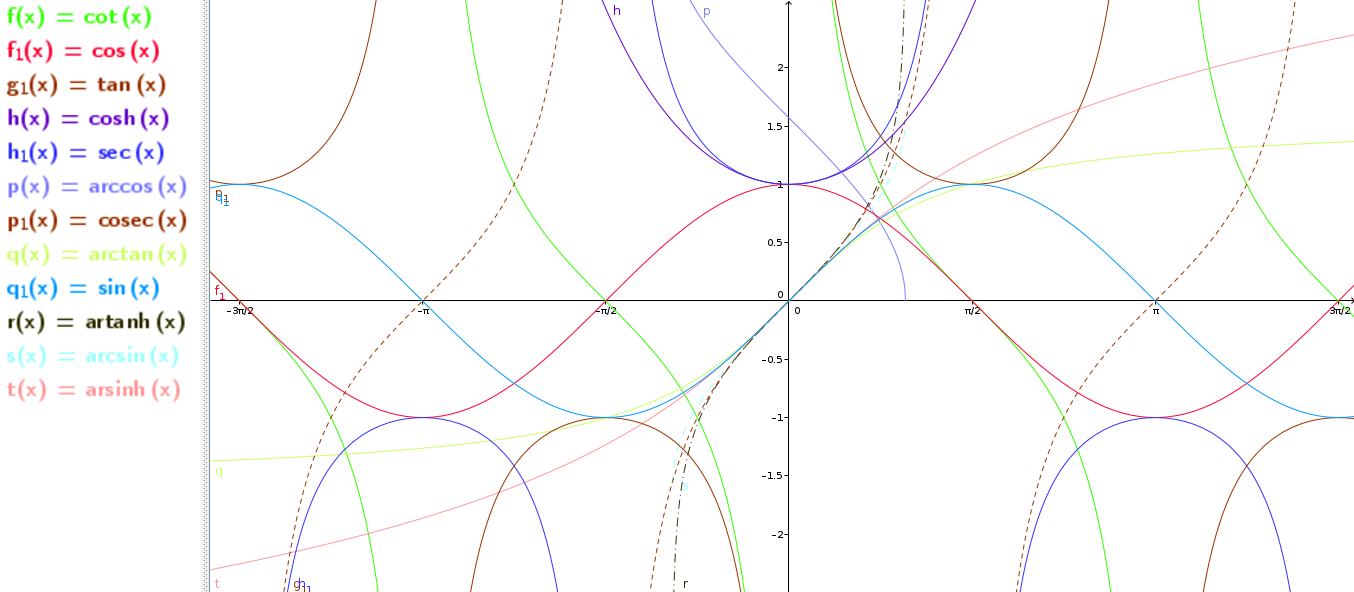
\includegraphics[height=8cm]{funktionen.png} \\
\includesvg[height=6cm]{Log4} \\
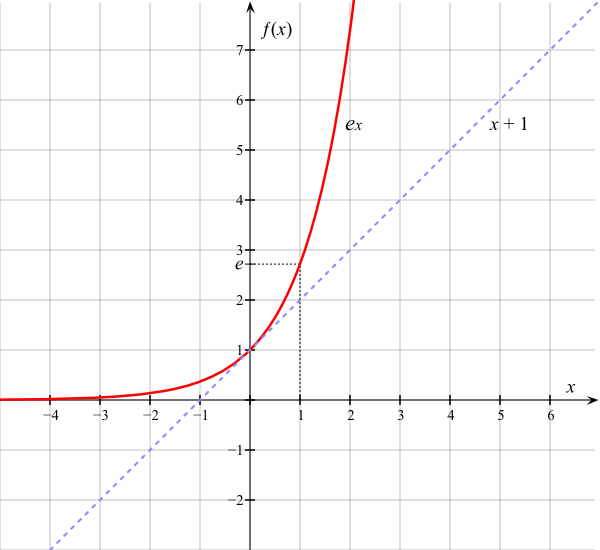
\includegraphics[height=6cm]{Exp_e.png} \\
\end{multicols}

% Ende der Spalten


% Dokumentende
% ======================================================================
\end{document}
